\documentclass{article}
\usepackage[utf8]{inputenc}

\title{\Huge Comptes rendus réunions n°6}
\author{Participants : Ridel Julien - Youssef Trabelsi - François Dénès \\ Durée : 4h}
\date{06/12/2021}

\usepackage{natbib}
\usepackage{graphicx}

\begin{document}

\maketitle

\section{\huge Déroulé de la séance}

\Large Utiliser la séance de TP du lundi 06/12/2021 pour mettre en place les bases de notre application afin de commencer le développement


\begin{itemize}

    \item \Large Réalisations de Julien Ridel :
    
    \begin{itemize}
        \item \Large Création d'une page très basique en html avec la mise en place d'éléments de style. La partie Flask n'a pas été abordée lors de cette séance. Le style de la page à été défini afin de donner une charte graphique à suivre pour tout le groupe.
        Un début de mise en place d'un futur bouton pour ajouter des posts sur notre application a été lui aussi ajouté.
    \end{itemize} 
    
     \item \Large Réalisations de Youssef Trabelsi :
    
    \begin{itemize}
        \item \Large Création d'un premier schéma relationnel afin de prévoir la future base de données qu'il faudrat implémenter à notre application. Le fichier draw.io de ce schéma est présent dans le dossier de ce compte rendu ainsi qu'une capture d'écran à la fin de ce document.
    \end{itemize} 
    
    \item \Large Réalisations de François Dénès :
    
    \begin{itemize}
        
        \item \Large Aide pour certains aspects de style de la page html.
        \item \Large Aide pour la réalisation du schéma relationnel puis vérification.
        \item \Large Recherche pour la mise en place d'un système permettant la création de fenêtre pop up sur notre page principale afin d'éviter une redirection sur une nouvelle page lors de la consultation d'un post.
    \end{itemize} 
\end{itemize}

\section {\huge Schéma relationnel réalisé par Youssef Trabelsi}

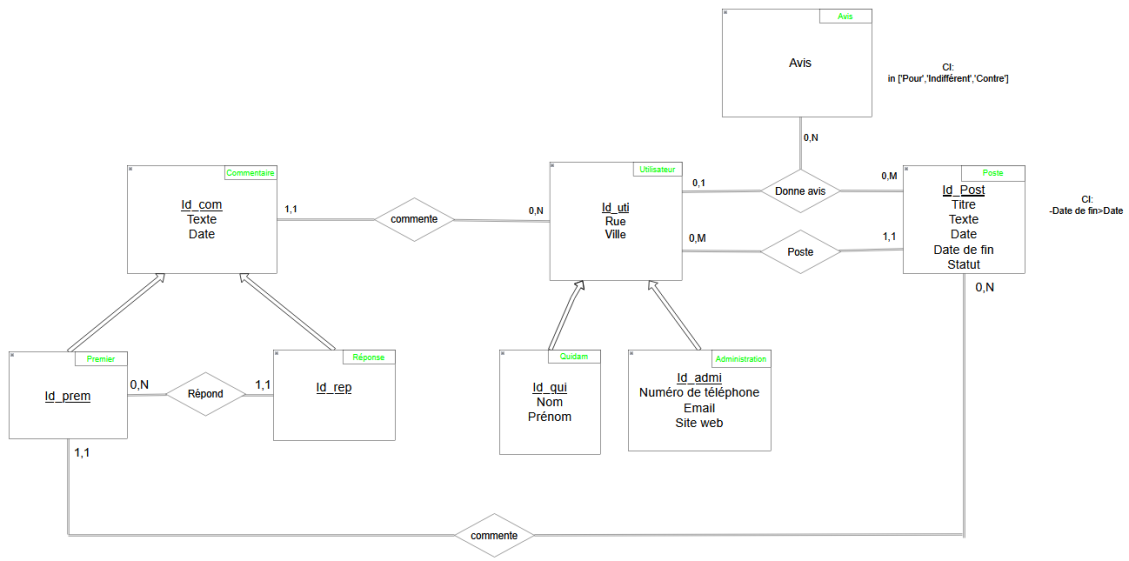
\includegraphics[scale=0.30]{Schema_relationnel.png}

\section {\huge Conclusion de fin de séance}

    \begin{itemize}
            \item \Large A la fin de cette séance, nous nous sommes mis d'accord sur le fait que lors des jours suivant, le développement allait être léger. En effet, nous avons voulu prendre du temps pour les partiels, quitte a devoir redoubler d'efforts par la suite. 
            Mais ceci n'était pas obligatoire, il est possible de commencer les recherches pour le développement de notre application.
    \end{itemize} 

\end{document}
